\documentclass[12pt, a4paper]{article}

%%%%%% 	pacotes	%%%%%%%
%\usepackage[utf8]{inputenc}
\usepackage[portuguese]{babel}
\usepackage[T1]{fontenc}
%\usepackage{fontspec} % habilita o comando /setmainfont{times new roman}
\usepackage{graphicx, wrapfig} % para importar imagens e para coloca-las ao lado do texto

\usepackage{amsmath, amsfonts, amssymb, amsthm, mathrsfs} %o penultimo para teoremas e o ultimo para o comando \mathscr{<texto>}

%\usepackage{blindtext} % para gerar textos com o comando \blindtext[1]

\usepackage[left=3cm,right=2cm,top=3cm,bottom=2cm]{geometry} % definindo as medidas das margens do papel
\usepackage{hyperref} % para fazer o sumario ficar interativo e adicionar hiperlinks
%%%%%%%	preambulo	%%%%%%
%\setmainfont{Times New Roman}
%\setlength{\parskip}{18pt} %18pt/12pt = 1.5, o padrao abnt. define a distancia entre linhas para ser 18pt, como se houvesse uma palavra de tamanho 18pt entre as linhas 
\setlength{\parskip}{0cm}
%\setlength{\parindent}{1.25cm} %define o recuo do paragrafo para ser 1.25cm (o padrao da norma ABNT)
\setlength{\parindent}{0cm}


\hypersetup{colorlinks=true, %set true if you want colored links
    linktoc=all,     %set to all if you want both sections and subsections linked
    linkcolor=red,  %choose some color if you want links to stand out
} %https://tex.stackexchange.com/questions/73862/how-can-i-make-a-clickable-table-of-contents


\theoremstyle{definition} \newtheorem{prob}{Problema}
\newtheorem*{res}{Resolução}

\begin{document}
\pagestyle{empty}

\begin{wrapfigure}{L}{0.1\textwidth} % o parametro L: a posição da imagem em relação ao texto: a esquerda do texto. outros valores: l, r, i, o, R, O, I. Já o segundo parametro indica o quao perto o texto esta da imagem. Mudar apenas o valor numerico
\includegraphics[width=0.065\textheight]{logo ufpe.jpg}
%separando cada linha por multiplos de 1.5cm, o espaçamento padrão segundo as normas da ABNT.

\end{wrapfigure}
\noindent UNIVERSIDADE FEDERAL DE PERNAMBUCO\\CENTRO DE CIÊNCIAS EXATAS E DA NATUREZA\\DEPARTAMENTO DE MATEMÁTICA\\PRINCÍPIOS DE CONTAGEM - 2023.1\\PROFESSOR: WILLIKAT BEZERRA DE MELO\\TURMA: 2Z\\

\begin{flushleft}

MONITOR: JARDEL FELIPE CABRAL DOS SANTOS\\[0.75em] 
\end{flushleft}

\begin{center}
\section*{\normalsize RESOLUÇÃO DA LISTA 7\\[0.25em]} 
\end{center}

\begin{prob} %problema 1
Desenhe um grafo completo com 4 vértices.

\dotfill
\begin{res}
\end{res}
\begin{center}
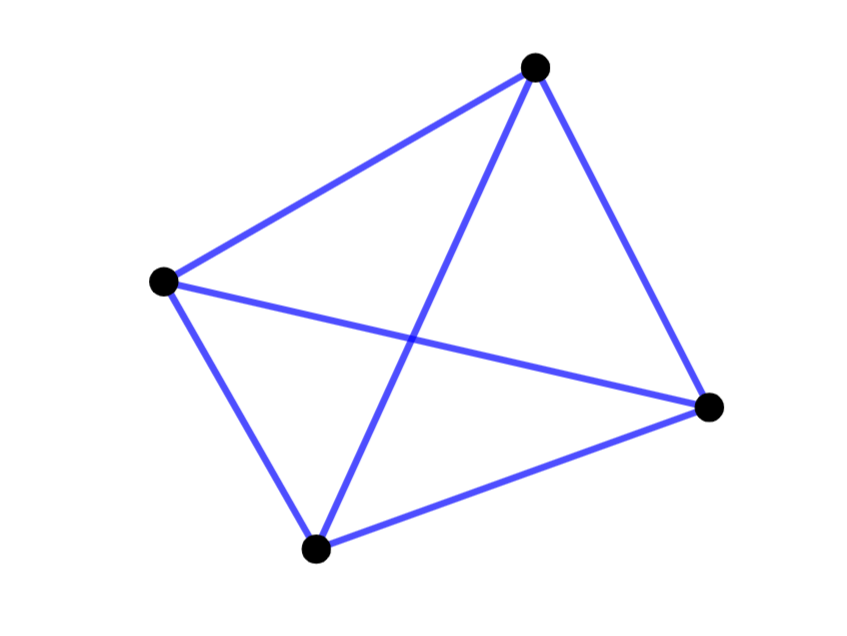
\includegraphics[scale=1]{gcompleto_4vertices.png}
\end{center}
\dotfill
\end{prob}

\begin{prob} %problema 2
Responda o que se pede.
\begin{enumerate}
\item[(a)] Dado um grafo \(G\) com vértices \(\{A, B, C, D, E\}\) e arestas \(\{(A,B), (B,C), (C,D), (D,E)\}\), indique um subgrafo desse grafo.
\end{enumerate}
\dotfill
\begin{res}
\end{res}
Utilizaremos a notação \(\mathrm{V}(X)\) para denotar o conjunto de vértices do grafo \(X\) e \(\mathrm{E}(X)\) para denotar o conjunto de arestas do grafo \(X\). \\

Por definição, um grafo \(H\) é subgrafo de um grafo \(G\) se \(\mathrm{V}(H) \subset \mathrm{V}(G)\) e \(\mathrm{E}(H) \subset \mathrm{E}(G)\).  Assim, podemos obter um subgrafo \(H\) de \(G\) se escolhermos \(\mathrm{V}(H) \subset \mathrm{V}(G)\) e \(\mathrm{E}(H) \subset \mathrm{E}(G)\) de modo que \(H\) seja um grafo. Por exemplo: \\

Se \(H\) é o grafo onde \(\mathrm{E}(H) = \{(A,B)\}\) e \(\mathrm{V}(H) = \{A,B,C,D\}\), então \(H\) é subgrafo de \(G\).

\dotfill

\begin{itemize}
\item[(b)] 
Explique a diferença entre subgrafo induzido e subgrafo não induzido.
\end{itemize}
\dotfill
\begin{res}
\end{res}
Dado um grafo \(G\) e conjunto \(X \subset \mathrm{V}(G)\), dizemos que o grafo \(H\) é o subgrafo de \(G\) induzido por \(X\) se \(\mathrm{V}(H) = X \) e \(\mathrm{E}(H) = \{(u,v): u, v \in X\}\). Se \(\mathrm{E}(H) \varsubsetneq \{(u,v): u, v \in X\}\), então dizemos que o subgrafo \(H\) é não é induzido por \(X\), ou seja, é não induzido.

\end{prob}
\dotfill

\begin{prob} %problema 3
Responda o que se pede.
\begin{enumerate}
\item[(a)] O que é uma árvore em teoria dos grafos?
\end{enumerate}
\dotfill
\begin{res}
\end{res}
Uma árvore é um grafo \(G\) que é acíclico e conexo.

\dotfill
\begin{enumerate}
\item[(b)] Desenhe uma árvore com 4 vértices.
\end{enumerate}
\dotfill
\begin{res}
\end{res}
\begin{center}
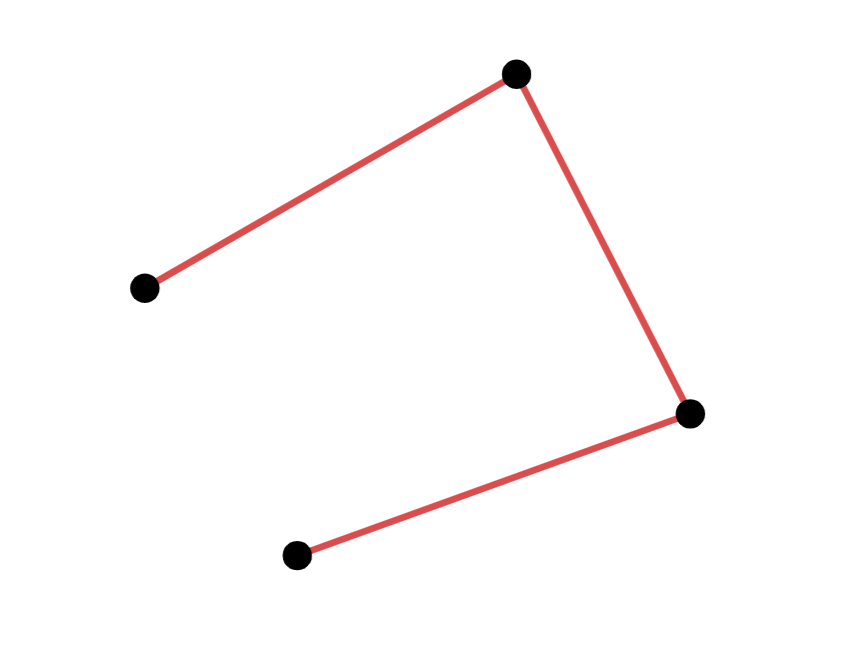
\includegraphics[scale=0.25]{arvore_4vertices.png}
\end{center}

\dotfill
\begin{enumerate}
\item[(c)] Qual é o número mínimo de arestas que uma árvore com \(n\) vértices pode ter?
\end{enumerate}
\dotfill
\begin{res}
\end{res}
\textbf{Afirmação:} Uma árvore com \(n\) vértices pode ter no mínimo \(n-1\) arestas. \\

Para demonstrar esta afirmação, precisaremos de dois teoremas: \\

\textbf{Teorema 1:} Se \(G\) é um grafo conexo com \(n\) vértices, então \(\mathrm{e}(G) \geq n-1\). \\

\textbf{Teorema 2:} Seja \(G\) um grafo conexo com \(n\) vértices. Se \(\mathrm{e}(G) = n-1\), então \(G\) é acíclico. \\

Estes teoremas aparecem nas \href{https://drive.google.com/file/d/16Gy9vck48p64A-3u1t2-uUVGOVqOlAOg/view}{notas de aula} e são demonstrados na página 41 e 42 da mesma. Ver lema 3 e proposição 8. \\

\begin{proof}[Demonstração da afirmação]
Faremos a demonstração em duas etapas: \\

(1) Mostrar a existência de uma árvore com \(n\) vértices e com \(n-1\) arestas.\\

(2) Argumentar que não existe árvores com \(n\) e com menos de \(n-1\) arestas.\\

Seja \(G\) um grafo conexo com \(n\) vértices. Pelo teorema 1, temos que \(\mathrm{e}(G) \geq n-1\). Ou seja, o número de arestas de \(G\) é pelo menos \(n-1\). Para ser uma árvore, \(G\) precisa ser acíclico. Suponha que \(\mathrm{e}(G) = n-1\) (o teorema 1 garante que isso é possível). Logo, pelo teorema 2, temos que \(G\) é acíclico. Portanto, por definição, \(G\) é uma árvore. Desse modo, existe uma árvore com \(n\) vértices e com \(n-1\) arestas. \\

Como toda árvore é um grafo conexo, então, dada uma árvore \(A\) com \(n\) vértices, pelo teorema 1, temos que \(\mathrm{e}(A) \geq n-1\). Logo, o número mínimo de arestas que uma árvore com \(n\) vértices pode ter é \(n-1\) arestas.
  
\end{proof}


\dotfill
\begin{enumerate}
\item[(d)] Quantas folhas uma árvore com 7 vértices pode ter no máximo?
\end{enumerate}
\dotfill
\begin{res}
\end{res}
Observe na figura a abaixo uma árvore com 7 vértices e 6 folhas: \\

\begin{center}
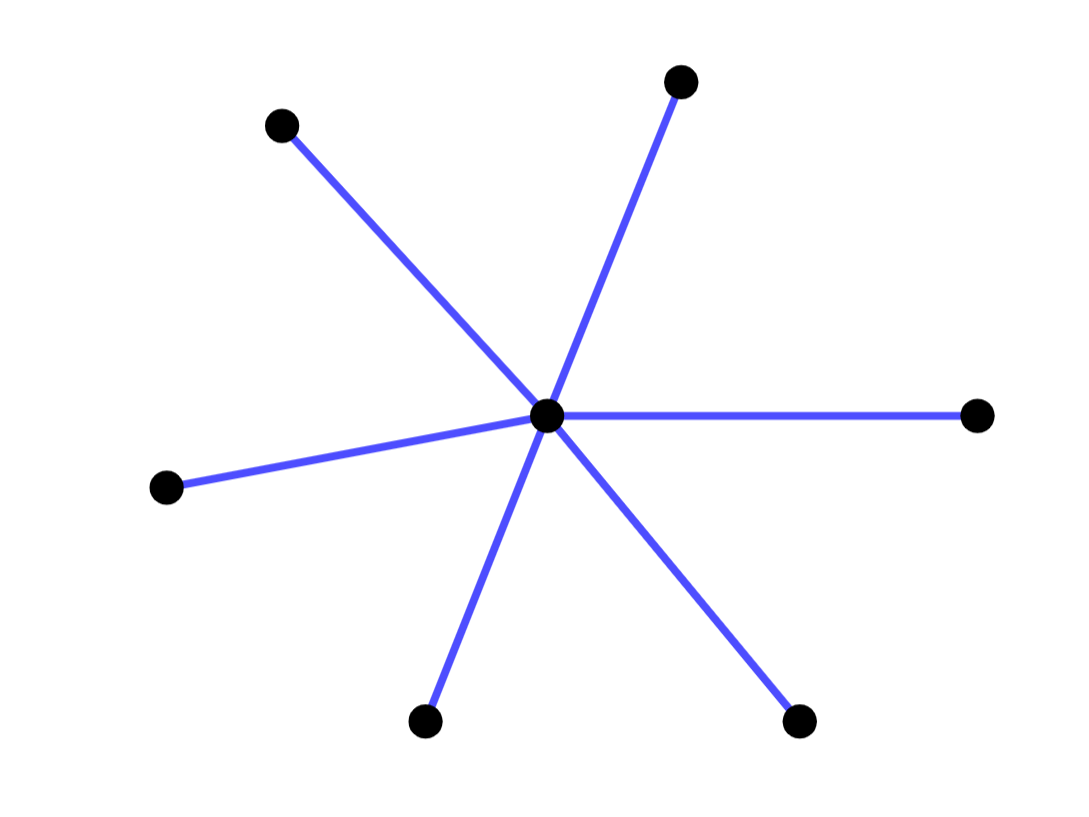
\includegraphics[scale=0.25]{arvore_6folhas.png}
\end{center}

\textbf{Afirmação:} Uma árvore com 7 vértices tem no máximo 6 folhas. \\


Para demonstrar esta afirmação, utilizaremos o seguinte lema: \\

\textbf{Lema:} Um grafo \(G\) é conexo se e somente se para quaisquer \(x,y \in \mathrm{V}(G)\), existe um caminho de \(x\) a \(y\). \\

Este lema aparece nas \href{https://drive.google.com/file/d/16Gy9vck48p64A-3u1t2-uUVGOVqOlAOg/view}{notas de aula} e é demonstrado na página 40 da mesma. Ver lema 2.

\begin{proof}[Demonstração da afirmação]
Suponha, para efeito de absurdo, que exista uma árvore \(G\) com 7 vértices e com mais de 6 folhas. Pela definição de folha, o número de vértices de grau 1 é igual à quantidade de folhas da árvore. Logo, \(G\) deve ter 7 folhas pois só possui 7 vértices. \\

Considere \(u,v,w \in \mathrm{V}(G)\) tais que \(u\neq v\), \(u \neq w\) e \(v \neq w\). Por ser uma árvore, temos que \(G\) é conexo. Desse modo, pelo lema, para quaisquer \(x,y \in \mathrm{V}(G)\), existe um caminho de \(x\) a \(y\).  Sejam \(A\) e \(B\) sequências de vértices de \(G\) que descrevem um caminho de \(u\) a \(v\) e \(u\) a \(w\), respectivamente. Temos duas possibilidades: \\

(i) ou a sequência \(A\) tem exatamente dois termos. (\(A = (u,v)\)) \\

(ii) ou a sequência \(A\) tem mais de dois termos.  \\

Note que (ii) não pode acontecer, pois implicaria que existe um vértice de \(G\) que tem grau maior do que 1 (esse vértice seria uma ``ponte'' que ligaria dois vértices no caminho) e contradiria a hipótese de \(G\) ter 7 folhas. Assim, necessariamente (i) deve acontecer. \\

De maneira análoga, podemos concluir que \(B\) é uma sequência com exatamente dois termos, ou seja: \(B =(u,w)\). Porém, isso significa que existem as arestas \(e_1 = \{u,v\}\) e \(e_2 =\{u,w\}\) na árvore \(G\) (caso contrário os caminhos entre os vértices não existiriam). Daí, pela definição de grau de um vértice, temos que o grau do vértice \(u\) é pelo menos 2. Desse modo, \(u\) não é uma folha de \(G\). Absurdo! pois supomos que todo vértice de \(G\) é uma folha.\\

O absurdo aconteceu pois supomos a existência das sequências de vértices \(A\) e \(B\). Logo, conclui-se que não existem tais sequências e, portanto, não existem caminhos de \(u\) a \(v\) e de \(u\) a \(w\). Assim, pelo lema, \(G\) não é conexo. Absurdo! pois supomos que \(G\) é uma árvore e toda árvore é conexa. \\

Conclui-se que tal árvore \(G\) não pode existir. Ou seja, não existe uma árvore com 7 vértices e mais de 6 folhas.

\end{proof}

\dotfill

\end{prob}

\begin{prob} %problema 4
Mostre que dados dois vértices \(u\) e \(v\) de um grafo \(G\), existe um caminho ligando \(u\) a \(v\) se e somente se existe um passeio ligando \(u\) a \(v\).

\dotfill
\begin{res}
\end{res}
Este problema aparece nas \href{https://drive.google.com/file/d/16Gy9vck48p64A-3u1t2-uUVGOVqOlAOg/view}{notas de aula} e é demonstrado na página 39 da mesma. Ver proposição 6.

\end{prob}
\dotfill
\begin{prob} %problema 5
Mostre que se \(G\) é um grafo com \(\delta (G) \geq 2\), então \(G\) contém um ciclo de comprimento pelo menos \(\delta (G) +1\).

\dotfill
\begin{res}
\end{res}
Este problema aparece nas \href{https://drive.google.com/file/d/16Gy9vck48p64A-3u1t2-uUVGOVqOlAOg/view}{notas de aula} e é demonstrado na página 39 da mesma. Ver proposição 7.

\dotfill
\end{prob}

\begin{prob} %problema 6
Mostre que toda árvore com \(n \geq 2\) vértices tem pelo menos duas folhas.

\dotfill
\begin{res}
\end{res}
Este problema aparece nas \href{https://drive.google.com/file/d/16Gy9vck48p64A-3u1t2-uUVGOVqOlAOg/view}{notas de aula} e é demonstrado na página 42 da mesma. Ver lema 4.

\end{prob}


\end{document}